\documentclass {article}

\usepackage[spanish]{babel}
\usepackage [T1]{fontenc}
\usepackage [utf8]{inputenc}
\usepackage {graphicx}
\usepackage{pdfpages}   %incluir paginas de pdf externo, para los anexos
\usepackage{appendix}
\usepackage{tikz}

\begin {document}

\title{Laboratorio 5}
\author{Daniel García Vaglio, B42781}
\maketitle
\begin{abstract}
Este es el documento explicativo correspondiente al quinto laboratorio
del curso de Circuitos Digitales 2.  Para este laboratorio se hace un
contador de 32 bits en descripción conductua, y se sintetiza con Yosys.
\end{abstract}


\section{Descripción Arquitectónica}

Para esta tarea se diseña un contador de 32 bits. Este se compone de 8
contadores de 4 bits, que se conectan entre ellos por medio de lógica
combinacional. Los contadores de 4 bits independientemente pueden
contar hacia adelante y hacia atrás de uno en uno, hacia atrás de 3 en
3 y recibir cargas paralelas.  En el caso del contador de 4 bits se
hacen casos para cada modo de conteo, y se describe el comportamiento
del resultado de cuenta y de RCO en cada caso.

Se tienen cuatro módulos. El primero es el contador, este es la
descripción conductual del contador. Luego se tiene el módulo de
señales.  Este se encarga de enviarle al contador las entradas
necesarias para que haga la cuenta. El tercer contador es el
verificador. Este se encarga de comparar la salida del contador
estructural y el conductual, y detener la simulación cuando no
coinciden. Por último el test bench es el módulo encargado de conectar
el resto.

\section{Plan de pruebas}

Primero se hace la síntesis del contador de 32 bits a la librería
general de Yosys. Y se hace la prueba de verificación de equivalencia
lógica. Esta cuenta consiste en primero cargar 0, luego contar hasta
$2^{16}$. Luego cargar $2^{32}$ y contar de forma regresiva hasta
$2^{16}$.  Luego se hace una cuenta de tres en tres regresiva por la
misma cantidad de tiempo. Se hace de esta manera para que el contador
pase por todos los valores posibles, y se pueda verificar que no hay
errores.

Luego se hace la síntesis con la librería cmos\_cells. Y se corre al
misma prueba de verificación. Si la simulación no se detiene, es que
no hubieron errores. Al final se debe digitar finish. la simulación no
termina automáticamente pera que se pueda revisar la salida.

Por último se tiene la prueba con retardo. En este caso se hace lo
mismo de cargar 0 y contar ascendentemente y luego se carga 0xFFFFFFFF
y se cuenta descendentemente, sin embargo para esta prueba no pasa por
todos los posibles valores, ya que sí se tiene la equivalencia lógica,
solo se hacen unos pasos para verificar que se tiene un resultado con
retraso. En este caso no se utiliza el verificador automático, porque
una señal está retrasada respecto a la otra, entonces da error cuando
no lo hay, pero sí se autoinicializa gtkwave, para visualizar las
formas de onda.

Se debe notar que existen dos contadores conductuales, uno es el
copnductual y al otro se le agrega \_for\_synthesis en el
nombre. Ambos son exactamente iguales, pero se hace el cambio de
nombre para evitar conflictos en el test\_bench. 

\section{Instrucciones}

Una vez descomprimida la tarea. En la raíz del directorio de la tarea
ejecute: make simple\_synthesis Este comando va a generar el contador
estructural a partir del conductual utilizando yosys.  Este comando lo
hace para la librería genérica de Yosys. Luego proceda a ejecutar:
make nodelay.  Esto va a correr la prueba de verificación de
equivalencia lógica entre los dos contadores existentes.  Al final de
la simulación ejecute finish. No se finaliza de forma automática para 
permitirle al usuario revisar en caso que hayan errores. 

Posteriormente, ejecute: make cmos\_synthesis. Este comando va a
sintetizar el contador estructural pero utilizando la biblioteca
cmos. Para hacer la prueba de equivalencia lógica, se ejecuta: make
nodelay.  Al final de la simulación ejecute finish. 

La tercera prueba es agregando los retardos. Para esto se tiene una
copia de la biblioteca cmos, pero con retardos. El comando make
delay\_synthesis se encarga de sintetizar un contador estructural,
pero utilizando la biblioteca con retardo. Se simula con el comando:
make delay.

Para Hacer la prueba de potencia ejecute: make power.

Puede ocurrir que al puro inicio de la simulación se reporte un error, solo se debe digitar cont. Esto es normal pues al principio las salidas son indeterminadas e Icarus Verilog las puede detectar como distintas. 

\section{Ejemplos de resultados}

Las pruebas de verificación de equivalencia lógica son exitosos. Como
se tiene el módulo verificador no es necesario utilizar gtkwave para
ver las formas de onda, y verificar manualmente que coinciden. Sin
embargo se incluyen los resultados en gtkwave para demostrar el
resultado en este reporte. En la figura \ref{fig:rtll} se muestra
el resultado de síntesis con compuertas genéricas. En la figura 
\ref{fig:cmos} se muestra el resultado de la simulación con síntesis
utilizando las compuertas cmos. Y finalmente los resultados de la 
simulación 

\begin{figure}[ht!]
  \centering
  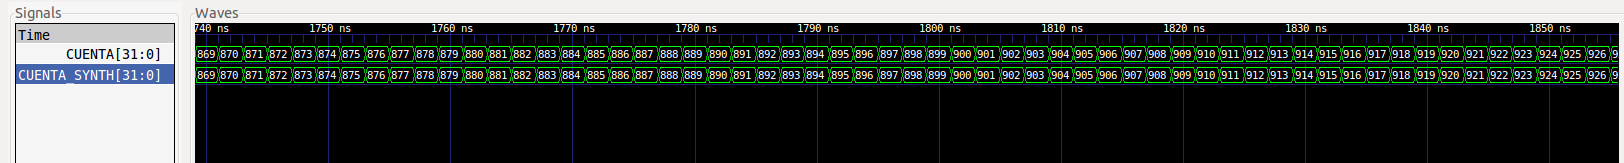
\includegraphics[width=0.7\textwidth]{./figures/gtkwave_rtll.png}
  \caption{Resultado de la simulación con biblioteca genérica}
  \label{fig:rtll}
\end{figure}

\begin{figure}[ht!]
  \centering
  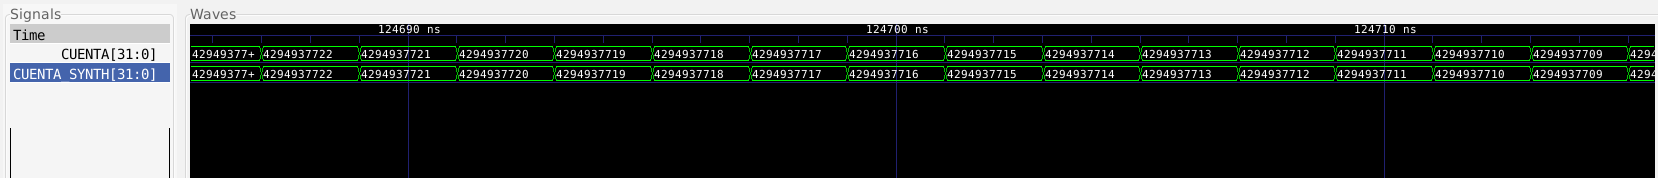
\includegraphics[width=0.7\textwidth]{./figures/gtkwave_cmos_lib.png}
  \caption{Resultado de la simulación con biblioteca cmos}
  \label{fig:cmos}
\end{figure}

\begin{figure}[ht!]
  \centering
  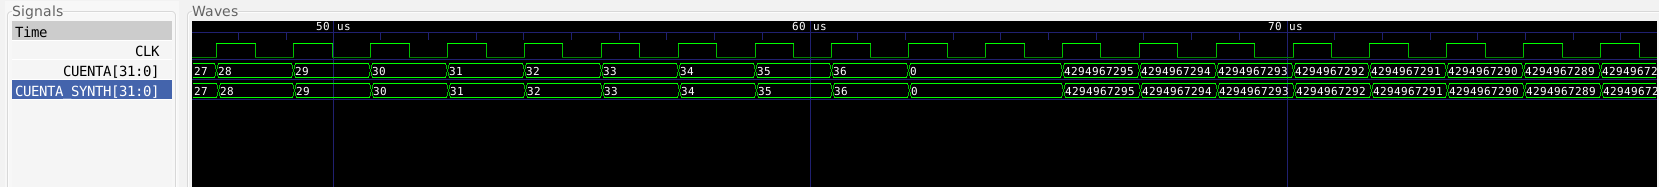
\includegraphics[width=0.7\textwidth]{./figures/gtkwave_delay.png}
  \caption{Resultado de la simulación con retardo}
  \label{fig:delay}
\end{figure}

\begin{figure}[ht!]
  \centering
  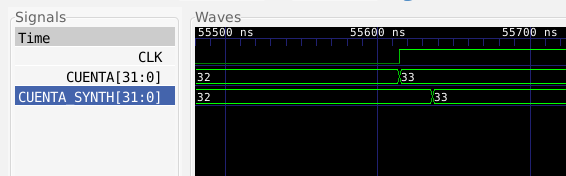
\includegraphics[width=0.7\textwidth]{./figures/gtkwave_restraso_entre_senales.png}
  \caption{Acercamiento a señal retardada}
  \label{fig:delay_zoom}
\end{figure}

\subsection{Frecuencia máxima}

Para determinar la frecuencia máxima se tomó la frecuiencia másima del
diseño anterior, y se comenzó a aumentar. Hasta llegar a un periodo de
$1612ns$, o $620347 Hz$. Para determinar la frecuencia límite, se
observaba el funcionamiento del circuito. Para periodos menores al
establecido el circuito no se comportaba correctamente.

\subsection{Potencia}

Respecto a la prueba de potencia se tiene que hay 1325125 conmutaciones en total. Como
el contador pasa por 12288 valores distintos y el periodo es de $1612ns$, entonces en total
se cuenta por $19808us$. La potencia viene dada por $220764968C$. 

\subsection{Costo}

Los contadores de 4 bits tienen 104 inverosres, y 92 NANDS. Entonces en total, tomando en cuenta la lógica del contador de 32 bits, se tienen 865 NOT, y 752 NAND. Esto implica comprar 217 componentes del inversor, y 189 NAND. Además de los 8 LATCH de 8 entradas. En total, se tienen 574 
dólares en componentes. 337135 dolones tomando en cuenta las horas que se invirtieron en el proyecto. 

\subsection{Comparación}
Se compara este contador de descripción estructural con el de la tarea pasada. Primero se debe hacer notar que este nuevo fue mucho más fácil de implementar, ya que no se necesitó
programar cada compuerta. Se ahorra mucho tiempo al hacer descripciones conductuales y luego utilizando Yosys. 

El nuevo circuito es más rápido, pues tiene caminos más cortos. El diseño anterior estaba dividido en módulos funcionales para facilitar su entendimiento, sin embargo esta facilidad para
el programador puede representar deficiencias en el desempeño. Yosys por otra parte procesa el contador como un todo, y  optimiza el circuito, entonces no se tiene ese problema. 

Este diseño no tiene multiplexores, entonces tiene mayor cantidad de compuertas. Esto lo hace más caro que el diseño anterior. Además consume más potencia. 

\section{Resultados y Conclusiones}

Se logra hacer la descripción conductual de un contador de 32 bits de, y luego sintetizarlo. Primero a utilizando una biblioteca genérica de componentes, luego con una biblioteca de CMOS, y finalmente con una biblioteca de cmos modificada, para tener retardos. Se logra comprobar la equivalencia lógica de la descripción conductual y la estructural. 

A continuación un resumen de los tiempos.

\begin{itemize}
\item Síntesis en biblioteca genérica, 30 min
\item Síntesis en biblioteca cmos, 2h 28 min (problema de los latches)
\item Modificación para retardos, 23 min
\item Síntesis con retardos, 5 min
\item Encontrar frecuencia mínima, 10 min
\item Código para contadores para la prueba de potencia, 25 min
\item Pruebas de potencia, 12 min
\item Cálculo de costo, 11 min
\item Escritura del reporte, 2h
\item total, 5h 24 min
\end{itemize} 


%\appendix
%\section{Anexos}

\end{document}
